% ****** Start of file main.tex ******
%
%
\documentclass[reprint,amsmath,amssymb,aps,pra]{revtex4-2}

\usepackage{graphicx}% Include figure files
\usepackage{dcolumn}% Align table columns on decimal point
\usepackage{bm}% bold math
%\usepackage{hyperref}% add hypertext capabilities
%\usepackage[mathlines]{lineno}% Enable numbering of text and display math
%\linenumbers\relax % Commence numbering lines

% \usepackage[%showframe,%Uncomment any one of the following lines to test 
% % scale=0.7, marginratio={1:1, 2:3}, ignoreall,% default settings
% % text={7in,10in},centering,
% margin=1.5in,
% total={6.5in,8.75in}, top=1.2in, left=0.9in, includefoot,
% height=10in,
% a4paper,
% hmargin={3cm,0.8in}
% ]{geometry}

\usepackage[utf8]{inputenc}
% \usepackage{hyperref}
\usepackage{braket}
\usepackage{physics}
\usepackage{amsmath,amssymb,amsthm}
\usepackage{tikz-cd}
\usepackage{enumerate}
\usepackage{xfrac}
\usepackage[parfill]{parskip}
\usepackage{subcaption}
% \usepackage{float}



% ####### New Commands #### %
\newcommand{\cm}{\mathbb{C}}
\newcommand{\re}{\mathbb{R}}

\newcommand{\proj}[1]{\ensuremath{{\ket{#1}\bra{#1}}}}
\makeatletter
\newcommand*\bigcdot{\mathpalette\bigcdot@{.8}}
\newcommand*\bigcdot@[2]{\mathbin{\vcenter{\hbox{\scalebox{#2}{$\m@th#1\bullet$}}}}}
\makeatother
\newlength{\arrow}
\settowidth{\arrow}{\scriptsize$1000$}
\newcommand*{\myrightarrow}[1]{\xrightarrow{\mathmakebox[\arrow]{#1}}}
\newcommand*{\TakeFourierOrnament}[1]{{%
\fontencoding{U}\fontfamily{futs}\selectfont\char#1}}
\newcommand*{\danger}{\TakeFourierOrnament{66}}
\setlength{\jot}{1.5mm}

\theoremstyle{definition}
\newtheorem{thm}{Theorem}[section] % the main one
\newtheorem{lemma}[thm]{Lemma}
\newtheorem{joke}{Joke}
% other statement types

% for specifying a name
\theoremstyle{plain} % just in case the style had changed
\newcommand{\thistheoremname}{}
\newtheorem{genericthm}[thm]{\thistheoremname}
\newenvironment{namedthm}[1]
  {\renewcommand{\thistheoremname}{#1}%
   \begin{genericthm}}
  {\end{genericthm}}
  
\newtheorem{defn}{Definition}
\newtheorem{prop}{Proposition}
\newtheorem{rmk}{Remark}
\newtheorem{conj}{Conjecture}
% \newtheorem{lemma}{Lemma}
\newtheorem{cor}{Corollary}
\newtheorem{problem}{Problem}

\begin{document}

\preprint{UW/PHYS-423/03-2021}

\title{Topological Phases of Matter}
\thanks{Nobel Prize 2016}

\author{Dan R. Mbanga}
\homepage{www.danulab.com}
\email{dmbanga@uw.edu}
\affiliation{University of Washington, Department of Physics} 
\altaffiliation[Also at ]{Amazon Web Services}

% Date
\date{\today}

%\keywords{Suggested keywords}%Use showkeys class option if keyword display desired

% Abstract
\begin{abstract}
    An article usually includes an abstract, a concise summary of the work
    covered at length in the main body of the article. 
    \begin{description}
    \item[Usage]
    Secondary publications and information retrieval purposes.
    \item[Structure]
    You may use the \texttt{description} environment to structure your abstract;
    use the optional argument of the \verb+\item+ command to give the category of each item. 
    \end{description}
    \end{abstract}

\maketitle

% \tableofcontents


% Introduction
\section{\label{sec:intro}Introduction}
The Nobel Prize in Physics 2016 was sahared among David J.Thouless (half of the prize), F. Duncan Haldane ($\frac{1}{4}$ of the prize), and J. Michael Korstelitz ($\frac{1}{4}$ of the prize), for \textbf{\textit{"theoretical discoveries of topological phase transitions and topological phases of matter"}}. The Nobel prize rewarded Thouless and Haldane for their contributions in understanding topological phases of matter \cite{thouless_quantized_1982}, and rewarded Korstelitz and Thouless for their contributions to understanding topological phase transitions \cite{kosterlitz_ordering_1973}. The idea could be simplified as: looking at an electron moving in a solid and exploring its wave function using topological concepts, one can explain a number of experiments. Kosterlit and Thouless introduced a new order parameter for phase transition based on principles of topology. They introduced a new definition of long range order based on golbal properties of a low-dimensional solid, as opposed to interactions between two points (spin-spin interactions for example) in the solid \cite{kosterlitz_ordering_1973}. This long range, "topological order" exists in 2D solids and neutral superfluids at a finite temperature, and is due to the proliferation of the unbinding of vortex-antivortex pairs also referred to as \textit{topological defects} in the 2D solid. 
% \textcolor{red}{In the case of a solid, the disappearance of topological long-range order is associated with a transition from an elastic to a fluid response to a small external shear stress, while for a neutral superfluid it is associated with the instability of persistent currents.} 
The idea of having a phase transition based on topological defects is now studied in many low-dimensional systems such as superfluid $^4He$, 2D Bose-Einstein condensates, superconductors.
\begin{description}
    \item[Order parameters vs topological invariants] what 
\end{description} 

% Electronic Matter background
\section{\label{sec:electronicMatter}Review of Electronic Matter}

Electronic matter \cite{haldane_model_1988} iss cool! \cite[testi]{fu_topological_2007}. Another example \cite[testi]{barber_phase_1980}

%Landay theory
\section{\label{sec:phases}Phase Transitions and Order Parameters}

The microscopic realization of a crystal reveals a lattice of ordered atoms. The lattice has a large $N$ number of atoms arranged in an ordered manner, with translational and rotational symmetry. To classify and explain the properties of materials, many theories were proposed. The \textit{principle of emergence} motivated the development of phenomenological methods to explain the properties of matter, which are based on a local \textit{order parameter} such as the magnetization $M$ for ferromagnetic phase transition as opposed to microscopic features such as spins, atoms, and molecules. These \textit{order parameters} characterize the organization of microscopic particles in the system, and are functions of coarse-grained variables such as temperatures and pressure. In his development of a theory of phase transition, Landau and Ginzburg \cite{hohenberg_introduction_2015,ter_haar_29_1965, wen_colloquium_2017} successfully associated different orders and hence different phases of materials, to different symmetries. He proposed that a discontinuity of the order parameter would cause a change of phase (or a phase transition), by spontaneously breaking the symmetry of the material. 

\begin{figure}[thpb] %this figure will be at the right
    \centering
    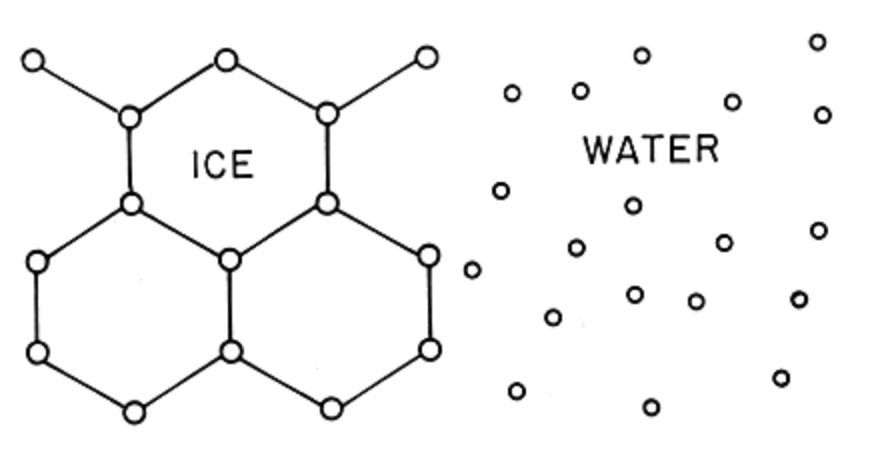
\includegraphics[width=0.25\textwidth]{figs/water-vs-ice.png}
    \caption{\label{fig:water-vs-ice}Ice breaks translational and rotational symmetries of water.}
\end{figure}

Crystals can be classified according to what types of symmetries are broken by their lattices. Crystals break translational and rotational symmetries of free space (e.g water losing translational and rotational symmetry by transition into ice). Liquid crystals only break the rotational symmetries. Magnets break time-reversal symmetry and the rotational symmetry of spin space. Superfluids (e.g low temperature $^{4}He$ at low temperature) break the $U(1)$ symmetry associated with the conservation of particles. 

%Topological phases of matter
\section{\label{sec:top-phases}Topological Invariants}

\subsection{\label{ssec:topo-intro}Topology in Physics}

Topology is the study of invariants under arbitrary continous transformations. 
A topological space can be thought of as a set from which has been swept away all structure irrelevant to the continuity of functions defined on it.

We now turn our attention to phases transitions in electronic matter that are not governed by an order parameter, but rather by a topological invariant.

\subsection{\label{ssec:landau-levels}Landau levels}
Feels like a SHO \\ 
$\ket{\Psi} \tens{R} \ket{\Phi}$ \\
$\partial_{x}A_{y}$ \\
$H = \dfrac{1}{2m}\left(P_{x} - \dfrac{q}{c}\left(-By\right)\right)^{2} + \dfrac{1}{2m}P_{y}^{2} + \dfrac{1}{2m}P_{z}^{2}$ \\ \\
$ \implies \left[H,P_{x}\right] = 0$ \\
$\therefore \psi(x,y) = \psi(y) e^{ik_{x}x}$ \\
$P_{x} = \hbar k_{x}$ \\
$H_{k_{x}} = \dfrac{P_{y}^{2}}{2m} + \dfrac{1}{2m}\left(\dfrac{qBy}{c} + \hbar k_{x}\right)^{2}  $ \\
$H_{k_{x}} = \dfrac{P_{y}^{2}}{2m} + \dfrac{1}{2} m \left(\dfrac{qB}{mc}\right)^{2} \left(y - \left(- \dfrac{\hbar k_{x} c}{qB}\right)\right)^{2} $ \\
$H_{k_{x}} = \dfrac{P_{y}^{2}}{2m} + \dfrac{1}{2} m \left(\dfrac{qB}{mc}\right)^{2} \left(y - y_{0}\right)^{2} $ \\
$y_{0} \equiv - \dfrac{\hbar k_{x} c}{qB}$

\subsection{\label{ssec:iqhe}The Integer Quantum Hall Effect (IQHE)}
$$
\boldsymbol{\sigma}=\left(\begin{array}{cc}
    0 & -\nu \frac{e^{2}}{h} \\
    \nu \frac{e^{2}}{h} & 0
    \end{array}\right)
$$


\subsection{\label{ssec:berry}Berry Phase}

\subsection{\label{ssec:tknn}TKNN}

\begin{align}
    & \mathbf{A}(\mathbf{k})=-i\left\langle u_{i}(\mathbf{k})\left|\nabla_{k}\right| u_{i}(\mathbf{k})\right\rangle \\
    &  \mathbf{F}(\mathbf{k})=\nabla_{k} \times \mathbf{A}(\mathbf{k}) \\
    & v=\frac{1}{2 \pi} \oint_{C} \mathbf{A}(\mathbf{k}) \cdot d \mathbf{k}=\frac{1}{2 \pi} \int_{B Z} \mathbf{F}(\mathbf{k}) d^{2} \mathbf{k}
\end{align}


%Examples and current work
\section{\label{sec:examples}Examples and Current Work}

%% Appendix %%
% \begin{acknowlegments}
% ACK HERE.
% \end{acknowlegments}

\appendix
\section{\label{app:a}Details 1}

\appendix
\section{\label{app:b}Details 2}

%% REFERENCES %%

% The \nocite command causes all entries in a bibliography to be printed out
% whether or not they are actually referenced in the text. This is appropriate
% for the sample file to show the different styles of references, but authors
% most likely will not want to use it.
\nocite{*}

\bibliography{topomatter}% Produces the bibliography via BibTeX.

\end{document}
%
% ****** End of file apssamp.tex ******
